\subsection{CMB temperature anisotropies: Sachs-Wolfe plateau}\label{sec:CMBSWPlateau}
Consider perturbations that are superhorizon at recombination, $k\tau_{rec}<1$. Recall that in Section~\ref{sec:SingCompFluid} we showed that $\delta \rho_m /\bar{\rho}_m = -2\Phi$ on superhorizon scales in a matter dominated Universe.
\underline{Assume that the perturbation is adiabatic}; i.e.\ the same for matter, radiation, cold dark matter and baryons:
\begin{equation}
    \frac{\delta \rho_m}{(\rho_m+p_m) } =\frac{\delta \rho_\gamma}{(\rho_\gamma+p_\gamma) } =\frac{3}{4}\frac{\delta \rho_\gamma}{\rho_\gamma} 
\end{equation}
and thus, at recombination (when Universe is matter dominated), $\frac{\delta \rho_\gamma}{\rho_\gamma} = -\frac{8}{3}\Phi$.

For these (high $\lambda$ $\rightarrow$ small $l$) modes, Sachs-Wolfe equation can be approximated by ignoring Doppler and time varying potential contribution:
\begin{equation}
    \frac{\Delta T_{now}}{T_{now}} (\mathbf{n}) \approx \frac{\delta \rho_\gamma}{4} (\tau_{rec}) + \Phi (\tau_{rec})= \frac{1}{3}\Phi(\tau_{rec})
\end{equation}

Again from Section~\ref{sec:SingCompFluid}, recall that $\Phi_{\mathrm{matter}} = (9/10) \Phi_{\mathrm{rad}} \, \Rightarrow \, \Phi(\tau_{rec})=(9/10)\Phi(\tau_{infl})$, as $\Phi(\tau_{infl}) \equiv \Phi(\tau_{i})$ is constant on superhorizon scales.
\begin{center}
    \begin{tikzpicture}
  \begin{axis}[
    width=10cm, height=5cm,
    xlabel={$\tau$},
    ylabel={$\Phi(\tau)$},
    ymin=0, ymax=1.2,
    xmin=0, xmax=4, 
    xtick={1.5,3},
    xticklabels={$\tau_{\rm eq}$,$\tau_{\rm rec}$},
    ytick={0.7,1},
    yticklabels={$\tfrac{9}{10}\,\Phi(\tau_i)$,$\Phi(\tau_i)$},
    domain=0:4,
    axis lines=middle, 
    clip=false,
  ]
    % initial plateau at unity
    \addplot[black, thick] coordinates {(0,1) (1.5,1)};
    % step down
    \addplot[black, thick] coordinates {(1.5,1) (1.5,0.7)};
    % second plateau
    \addplot[black, thick] coordinates {(1.5,0.7) (4,0.7)};
  \end{axis}
\end{tikzpicture}
\end{center}
Therefore, 
\begin{equation}
     \frac{\Delta T_{now}}{T_{now}} (\mathbf{n}) \approx \frac{3}{10}\Phi(\tau_i) = \frac{3}{10} \int \frac{d^3k}{(2\pi)^{3/2}}\Phi(\mathbf{k},\tau_i) e^{i \mathbf{k}\mathbf{n}r_*}
\end{equation}
As before expand the plane wave in Legendre polinomials to reach
\begin{eqopt}[darkred]\label{eq:ClApprox}
    C_l = \frac{36 \pi}{100} \int \frac{dk}{k} \Delta_{\Phi}(k) j^2_l (k r_*)
\end{eqopt}
with \textcolor{darkgreen}{$\Delta_{\Phi}(k) \equiv \frac{k^3}{2 \pi^2} P_{\Phi}(k)$}. Then define \textcolor{darkgreen}{$\Delta_{\Phi}(k) \equiv \left(\frac{k}{k_*}\right)^{n_s-1} \mathcal{A}_{\Phi}$}. With \textcolor{darkred}{$n_s \approx 1$},~\eqref{eq:ClApprox} gives
\begin{eqopt}[darkred]
    C_l=\frac{18 \pi}{100} \frac{\mathcal{A}_\Phi}{l(l+1)}
\end{eqopt} 
For small $l$ values, CMB data yelds
\begin{eqopt}[blue]
    \frac{l(l+1)C_l}{2\pi} \sim 10^{-10} \quad\textcolor{black}{\Rightarrow \quad \mathcal{A}_\Phi \approx 10^{-9}}
\end{eqopt}

\begin{figure}[h]
      \centering
        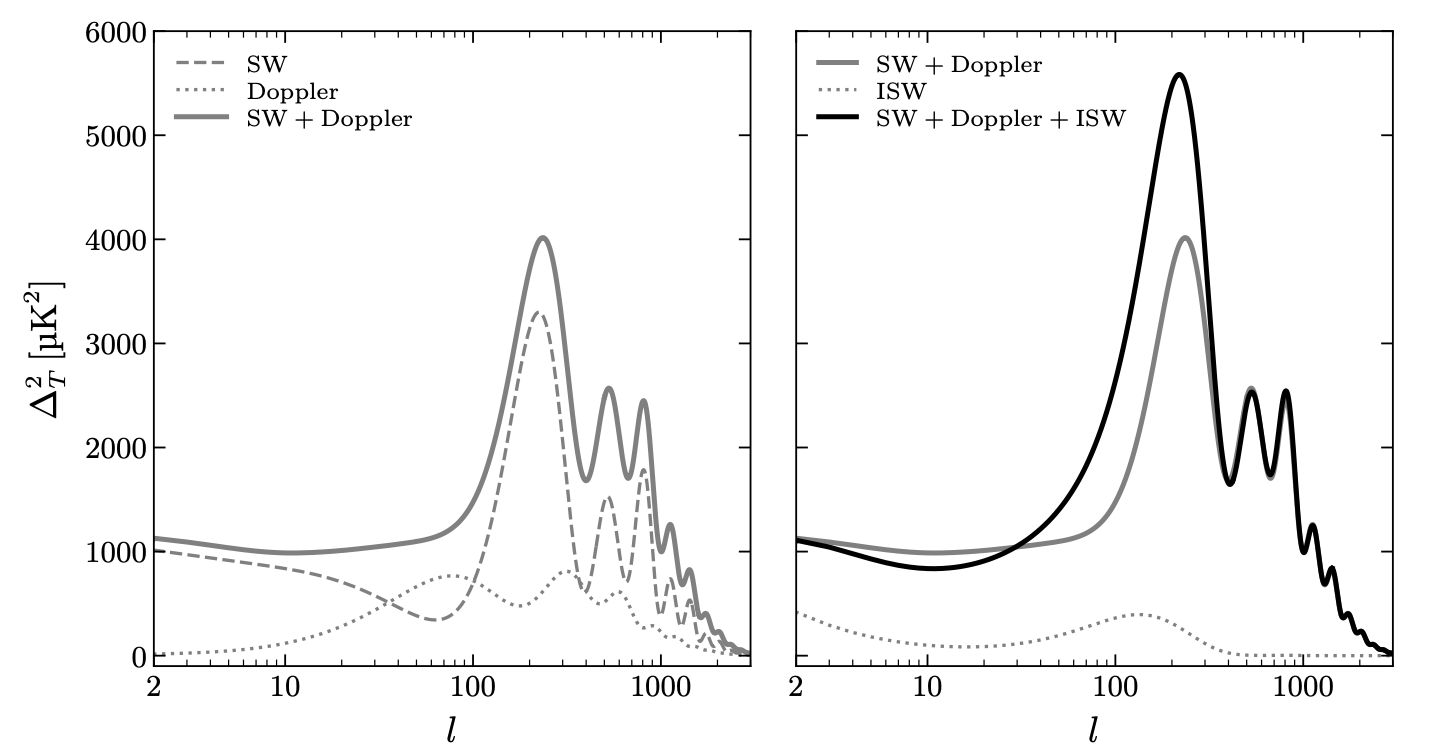
\includegraphics[width=0.8\textwidth]{Graphics/CMB.png}
        \caption{Sachs-Wolfe plateau characterizes the CMB angular spectrum for small $l$ values~\cite{CosmologyBau}.}
  \end{figure}

We can use this bound to constrain the scale of inflation. On superhorizon scales, the comoving curvature perturbation $\mathcal{R}=-u/z$ is $\approx$ \textcolor{darkgreen}{$\mathcal{\xi} \equiv -\Phi + \delta \rho /3(\rho+p)$}. The latter being the \textit{uniform density curvature perturbation}, i.e.\ the curvature perturbation measured on hypersurfaces where the total energy density is unperturbed.
In a radiation dominated Universe, as it is during inflation, $\xi= -\frac{3}{2}\Phi$.  
\begin{equation}
    \mathcal{R} \approx \mathcal{\xi}= -\frac{3}{2}\Phi \quad \Rightarrow \quad \Delta^2_{s} = \frac{9}{4} \Delta_{\Phi} \quad \Rightarrow \quad \mathcal{A}_{s} = \frac{9}{4}  \mathcal{A}_\Phi \approx 2\cdot 10^{-9}
\end{equation}
This implies $H^2/(8\pi^2 \epsilon)\approx 2\cdot 10^{-9} \;\Rightarrow\; H\simeq 10^{-4} \sqrt{\epsilon} \,M_P$.